\chapter{Introduction}
\label{ch:introduction}

\section{Background and Motivation}
\label{sec:background}

Greenhouse cultivation offers a controlled environment in which temperature, irrigation,
lighting and nutrient delivery can be regulated more directly than in open-field
agriculture. Hydroponic production adds precise control of the nutrient solution and
allows crops to be cultivated in structured rows. Despite this level of environmental
control, operations requiring physical interaction with individual plants and fruits
remain challenging to automate. Inspection, selective harvest, handling of delicate
produce and plant-care operations require the operator to combine visual assessment,
spatial reasoning and careful manipulation. These actions are repetitive, but their
physical details change with fruit position, orientation, size, occlusion and plant
growth.

A robotic platform that can move between planting rows, identify relevant objects and
interact with them carefully could reduce the manual workload and make operations more
consistent. However, agricultural manipulation cannot be treated as a conventional
industrial pick-and-place task with rigid, precisely located parts. Fruits are deformable,
can be hidden by leaves or neighboring produce, and may be damaged by excessive contact
forces or an unsuitable approach direction. A major review of harvesting robots
identifies crop-environment variability, robot capability and meaningful performance
measurement as key obstacles to practical harvesting systems \cite{bac2014}.

The present project therefore investigates a modular autonomous mobile manipulator for
hydroponic greenhouses. Rather than claiming a fully operational harvesting robot at the
current stage, the work focuses first on developing and testing the subsystems needed for
a future integrated prototype: mobile support, manipulator modeling, perception,
coordinate transformation, motion generation, compliant grasping and safety monitoring.
Digital simulation is used to evaluate candidate behaviors before transferring them to
the physical Lexium Cobot platform.

\section{Problem Statement}
\label{sec:problem}

The central engineering problem is to coordinate sensing, motion and contact in a system
that must act on objects whose exact positions and properties are not known beforehand.
A usable solution needs to solve several related problems. First, fruits must be detected
in camera images and localized in three-dimensional coordinates. Second, these coordinates
must be transformed into the manipulator reference frame with known calibration and
mounting geometry. Third, the robot must choose a reachable grasp pose and generate a
trajectory that respects joint limits, available clearance and relevant dynamic
constraints. Fourth, the end-effector must contact fragile produce with sufficiently
controlled force to maintain a stable grasp without causing damage. Finally, these
operations must be coordinated with the mobile base, fault detection and recovery
procedures.

A result demonstrated solely in a simulated scene is not necessarily reproducible on
real hardware. Mass and friction estimates, actuator constraints, visual noise,
calibration errors, deformable contact and timing differences can all affect behavior.
Consequently, the project distinguishes between software verification, physics-based
simulation experiments and physical-robot evaluation. This distinction also determines
how experimental evidence is reported in the present draft.

\section{Aim, Objectives and Scope}
\label{sec:objectives}

The overall aim is to develop a control system for an autonomous mobile manipulation
complex capable of assisting agricultural operations in hydroponic greenhouses, with a
particular focus on vision-guided, low-force fruit handling. The longer-term application
includes inspection, ripeness assessment, crop statistics and selective harvesting.
For the engineering development stage documented here, the objectives are:

\begin{enumerate}[label=\arabic*.]
 \item Model the Schneider Electric Lexium Cobot and the four-finger gripper, including
       kinematics, relevant joint constraints and collision geometry, in a simulation
       environment that can be used for repeatable testing.
 \item Establish a perception pipeline for fruit or proxy-object detection and
       three-dimensional localization using RGB and depth information.
 \item Define camera, gripper, manipulator and mobile-base coordinate frames, and
       prepare an eye-in-hand calibration procedure for transforming target locations
       into the robot workspace.
 \item Develop reachable approach, grasp, transfer and placement motions, together
       with safe startup, limit checking, rejection and recovery behaviors.
 \item Evaluate manipulation behavior in simulation using explicit success criteria,
       positioning errors, joint-motion limits and modeled contact forces.
 \item Integrate validated subsystems with physical hardware and, subsequently, with
       the mobile navigation system for greenhouse demonstrations.
\end{enumerate}

The project scope intentionally separates the final application from the currently
verified prototype functions. Color- and size-based sorting of simulated tomatoes is a
useful intermediate benchmark for perception, grasping and placement; it does not by
itself demonstrate plant inspection, detachment of fruit from stems, autonomous navigation
or an undamaged harvest on real plants. Those capabilities remain integration and
validation objectives.

\section{System Overview and Architecture}
\label{sec:architecture}

The proposed robot consists of an omnidirectional wheeled mobile base with an
aluminium-profile support frame, a six-axis Schneider Electric Lexium collaborative
manipulator and a four-finger compliant gripper. The project documentation specifies an
Intel RealSense RGB-D camera in an eye-in-hand arrangement near the end-effector. The
mobile base supplies movement between greenhouse rows, while the manipulator positions
the end-effector for inspection and handling. The compliant gripper is intended to
accommodate variations in object dimensions and contact geometry. Soft-gripper research
shows why contact adaptation and material compliance are relevant to grasping irregular
and fragile objects \cite{shintake2018}.

The intended control architecture is modular. ROS~2 provides a communication framework
for exchanging perception results, robot state, motion commands and navigation messages.
ROS~2 is suitable for such compositions because it supports distributed robotics
components and well-defined communication interfaces \cite{macenski2022}. Modules for
perception, transforms, manipulation planning, safety monitoring and task sequencing
can be tested separately and then connected. The digital twin provides an intermediate
stage in this integration, not a substitute for real-world calibration.

The intended manipulation sequence is as follows: the mobile platform approaches a
planting row; the camera acquires color and depth measurements; the perception module
returns candidate fruit objects and their estimated poses; the transform pipeline
expresses targets relative to the manipulator base; the planner evaluates reachable
approach and transfer paths; the gripper attempts controlled contact; the target is
placed in the designated container; and the supervisory logic confirms completion or
initiates recovery. This is the proposed end-to-end behavior, whereas only subsets of
it have currently been tested together.

\begin{figure}[htbp]
\centering
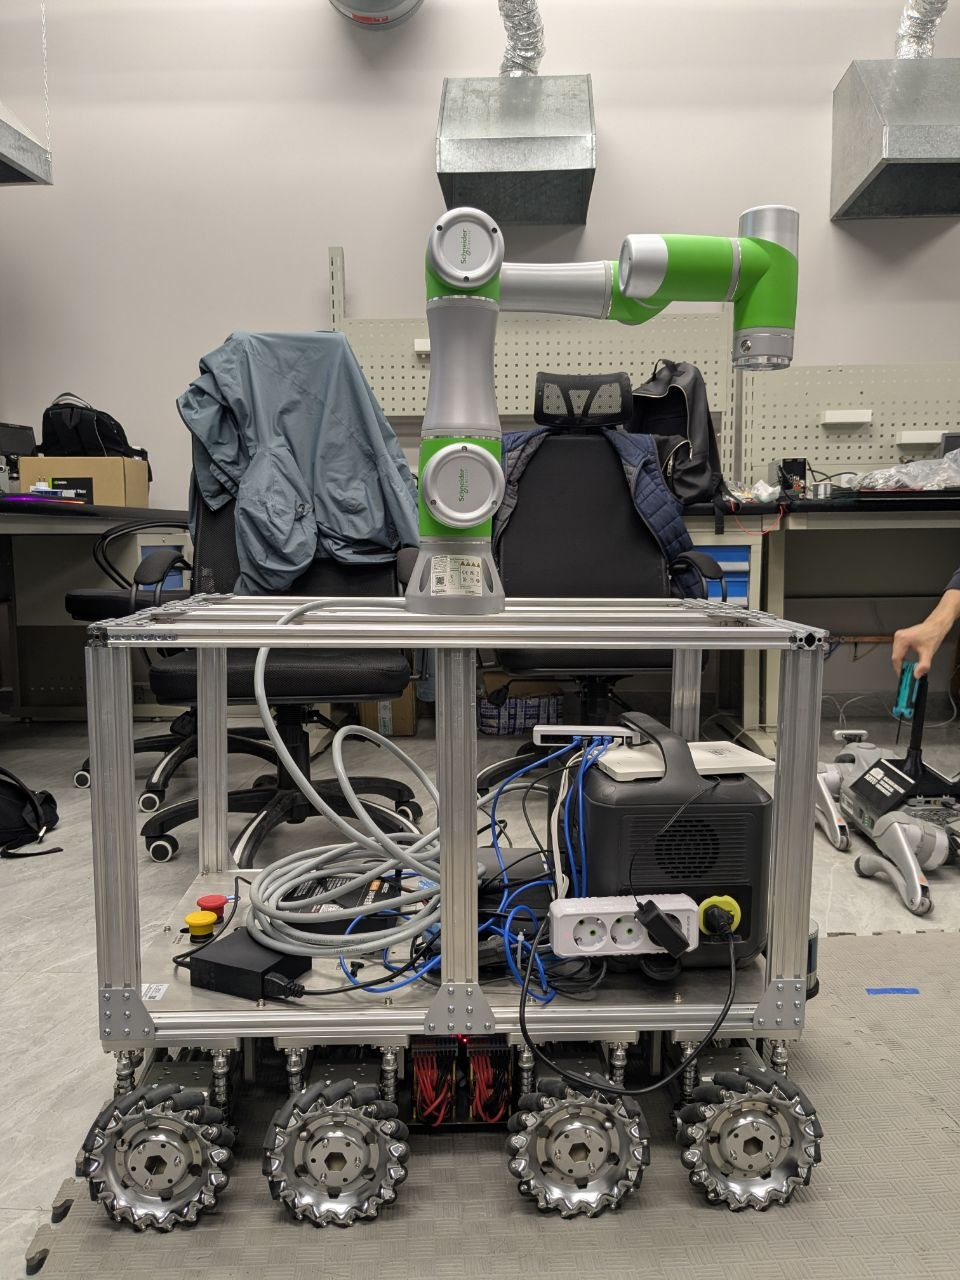
\includegraphics[width=0.81\linewidth]{mobile_platform.jpg}
\caption{Physical prototype platform showing the mounted Lexium Cobot and the omnidirectional wheeled base. The photograph documents mechanical assembly; it does not establish autonomous navigation or harvesting performance.}
\label{fig:mobile-platform}
\end{figure}

\section{Digital Twin, Perception and Manipulation Methodology}
\label{sec:methodology}

The software-development approach begins with the manipulator's geometric model and
its joint representation. The robot description and collision geometry are prepared
for simulation, and representative motions are checked against kinematic reachability,
mechanical limits and predicted actuator demands. NVIDIA Isaac Sim is used to visualize
and evaluate manipulation tasks with articulated rigid-body dynamics and contacts.
Isaac Lab supplies a related environment for robot-learning and policy-evaluation
workflows \cite{mittal2025}. At the time of writing, the provided test logs establish
simulation-level control and validation results, but they do not independently verify
a particular reinforcement-learning training run, reward curve or learned-policy
advantage. Any such performance claim requires the corresponding training artifacts.

For object perception, earlier experiments tested color segmentation, geometric
contours and depth-based localization with colored proxy objects. Later simulated
autonomous handling runs identify a TinyUNet-based perception component. This
combination supports a staged approach: visual detection produces a candidate object
or mask, depth sensing provides geometric information, and calibrated coordinate
transforms permit conversion from camera measurements to robot targets. A calibrated
camera mounted near the end-effector is envisaged for physical tests, but the full
Lexium-specific hand--eye calibration remains an outstanding milestone.

The manipulation pipeline performs task-state transitions rather than issuing isolated
motion commands. Startup and readiness checks establish a valid initial configuration;
object-localization and grasp planning precede contact; placement is verified before
advancing to another target; and infeasible or unsafe goals can be rejected. Tests
reported in the supplied validation suite cover both normal processing and rejection
and recovery. Safety constraints considered in simulation include joint configuration
margins, joint-speed bounds, trajectory feasibility, torque-model checks and limits on
modeled contact forces. These checks improve confidence in the digital experiment but
must be re-established on the actual hardware.

\section{Preliminary Implementation and Verification Status}
\label{sec:progress}

The physical evidence available for this progress review includes the assembled
omnidirectional base, the Lexium Cobot mounted on an aluminium-profile structure and
a four-finger gripper fitted to the robot wrist. Separate manual grasp demonstrations
with cylindrical bottles show geometric adaptability, although payload, object damage,
contact-force measurement and autonomous operation on hardware are not yet formally
validated. The available footage of the platform and manipulator supports a report
of integration work rather than completed agricultural field trials.

The project also includes a simulation validation suite executed on 17~November~2026.
Five named scenarios returned successful outcomes: (A) safe startup to ready state;
(B) handling a single simulated tomato with a TinyUNet perception component and the
four-finger gripper; (C) autonomously sorting three simulated tomatoes; (D) handling
randomized reachable target positions; and (E) rejecting an unsafe condition and
recovering. For the single-tomato scenario, the logged localization and placement
errors were 1.97~mm and 12.81~mm, respectively. For the three-target scenario, the
reported result was three successful picks out of three targets, with a localization
error of 3.10~mm and a reported contact-force value of 2.32~N. Two placement errors
of 9.65~mm and 17.64~mm were recorded in the randomized-position scenario.

A separate Stage~6 simulated sorting demonstration ended with five detected and five
sorted objects, and the supplied benchmark plot reports 100\% rates on five benchmark
categories in that selected test set. The display reports a contact value of 1.91~N
at completion, and a separate per-finger force chart depicts a simulation force
ceiling of 2.80~N. These numbers describe different views or runs and should not be
interpreted as the same measurement. The five-object benchmark should not be generalized
to an untested distribution of fruit sizes, appearances or greenhouse conditions.

\begin{figure}[htbp]
\centering
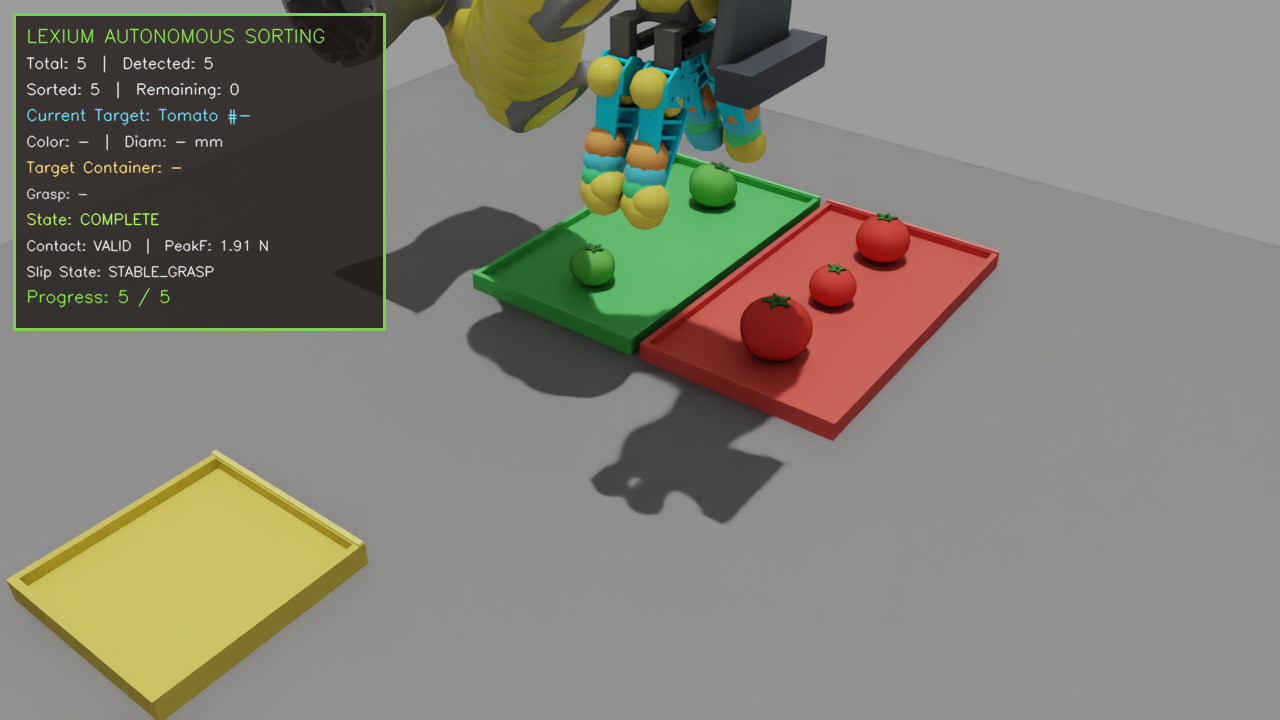
\includegraphics[width=0.92\linewidth]{stage6_sorting_scene.png}
\caption{Stage~6 Isaac simulation screenshot: five simulated tomatoes marked as detected and sorted. This is a software demonstration, not a physical sorting experiment.}
\label{fig:stage6-sorting}
\end{figure}

The hardware-constrained motion validation recorded 10,717 trajectory samples,
a maximum joint velocity of 0.593~rad/s, a maximum torque of 62.71~N\,m under the
URDF-based model, a maximum of 22.96~N\,m under the stated hardware-oriented torque
model and a minimum margin of 29.98\textdegree{} to the relevant joint limit. These
are model-dependent quantities and not measured joint torque on the physical cobot.
The automated software check reported 20 of 20 unit tests passed, while the deliverable
verification reported 21 of 21 items present. These results substantiate the
repeatability of the supplied software checks within their specified scope; broader
real-world reliability remains an open research question.

\section{Evaluation Criteria and Limitations}
\label{sec:evaluation}

Meaningful evaluation requires reporting more than a binary ``success'' flag. The
preliminary criteria are: object-detection or localization performance for a specified
test set; spatial error between commanded and achieved target positions; successful
pick-and-place completion; contact-force behavior during grasping; compliance with
robot-joint limits and motion constraints; task duration; and recovery from an unsafe
or infeasible request. For physical experiments, these criteria must be expanded to
include calibrated force measurements, real robot tracking error, repeated trials,
produce-damage assessment, and the effect of occlusions and changing illumination.

The available results have several limitations. All reported numerical localization,
contact and sorting benchmarks are derived from the supplied simulation results or
software-based tests. No quantitative physical fruit-damage data, field success rate,
real-world repeatability estimate or independently verified RL training curves were
included among the source materials. Furthermore, simulated contact forces depend on
collision geometry, material parameters and solver configuration. Such estimates cannot
be used as proof of gentle contact on actual fruit. Reporting these distinctions is
necessary for a defensible interpretation of project progress.

\section{Expected Contributions and Thesis Organization}
\label{sec:contributions}

The intended technical contribution is an integrated, modular control architecture
connecting perception, safe robot motion and compliant manipulation on a mobile base.
Interim engineering outputs include a physical mobile-manipulator assembly, a simulation
model of the manipulator and gripper, perception and calibration experiments, and
repeatable multi-scenario simulation checks. Further contributions will depend on
successfully transferring these capabilities to physical manipulation and, later, to
a coordinated mobile greenhouse trial.

The planned thesis will continue with a related-work review on greenhouse harvesting,
RGB-D perception, compliant end-effectors and robot control; a detailed description of
the mechanical and software architecture; robot kinematics and calibration methods;
experimental design and simulation/physical validation results; and an assessment of
limitations, safety and future development. This interim submission contains the
English Abstract and the Introduction required for the thesis-writing progress review;
other chapters are reserved for subsequent evidence-based development.
